\newpage
\section*{Problem 4:}
\begin{enumerate}
\item Function \texttt{run_gmres} is implemented as a wrapper around MATLAB \texttt{gmres} function so that we can plot the results and report the different statistics after the computation. File \texttt{problem_4.m} contains the driver that loads the two given matrices and run \texttt{run_gmres} on a loop that goes over all the cases. \texttt{run_gmres} outputs the relative residual norms, final approximate solution. Matrix-vector is inputted to \texttt{gmres} as routine that implements the matrix-vector multiplication in addition to counting how many times it's being called and reports it at the end of each case. For preconditioning cases, interested user might need to multiply the output $x_{k}$ from the left by $M1^{-1}$ to get the right results. We did not implement this since it is not used anywhere after the computation. 

\item Table~\ref{tab:mat1} and Figure~\ref{fig:mat1} show the results of running \texttt{gmres} for the different cases on \texttt{HW3_P4_1.mat} . Similarly, Table~\ref{tab:mat2} and Figure~\ref{fig:mat2} show the results for \texttt{HW3_P4_2.mat}. In the tables, we print out the output of the \texttt{iter} parameter as provided by MATLAB \texttt{gmres} function which shows the outer and
the inner iteration numbers at which final $x_{k}$ was computed.

\begin{figure}[tbh]
 \centering    
\begin{tabular}{ |p{6cm}|| p{1cm}|p{1.5cm}|p{1.5cm}|p{1.8cm}|p{1.7cm}|}
 \hline
Case & $k$ & Outer  & Inner &  \# GMRES  &\#  MatVec \\ \hhline{|=|=|=|=|=|=|}
 \hline
 (i) w/o Precondition                        &   & 1 & 103 & 103 & 105  \\
  \hline
 (ii) Restart w/o Precondition               & 5 &  42 & 5 & 211 & 253  \\                              
                                             & 10 & 26 & 5 & 256 & 282 \\
                                             & 20 & 18 & 1 & 342 & 360 \\                               
 \hline
(iii) Diagonal Precondition                  &   & 1 & 103 & 104 & 105 \\                              
 \hline
(iv) Restart Diagonal Precondition           & 5  & 42 & 5 & 211 & 253 \\                              
                                             & 10 & 26 & 5 & 256 & 282 \\
                                             & 20 & 18 & 1 & 342 & 360 \\
 \hline
(v) Precondition From 3, $D=D_{0}$           &   & 1 & 30 & 31 & 32  \\                              
 \hline
(v) Precondition From 3, $D=10I$             &   & 1 & 41 & 42 & 43 \\                              
 \hline
(vi) Restart Precondition From 3, $D=D_{0}$  & 5  & 13 & 3 & 64 & 77  \\                              
                                             & 10 & 8  & 5 & 76 & 84 \\
                                             & 20 & 2  & 18& 39 & 41 \\
\hline
(vi) Restart Precondition From 3, $D=10I$    & 5  & 19 & 3  & 94  & 113  \\                              
                                             & 10 & 13 & 10 & 131 & 144  \\
                                             & 20 & 7  & 1  & 122 & 129 \\
 \hline
\end{tabular} 
\caption{Results for input matrix from \texttt{HW3_P4_1.mat}}
   \label{tab:mat1}
\end{figure} 


\begin{figure}[!tbh]
\centering        
   \subfloat{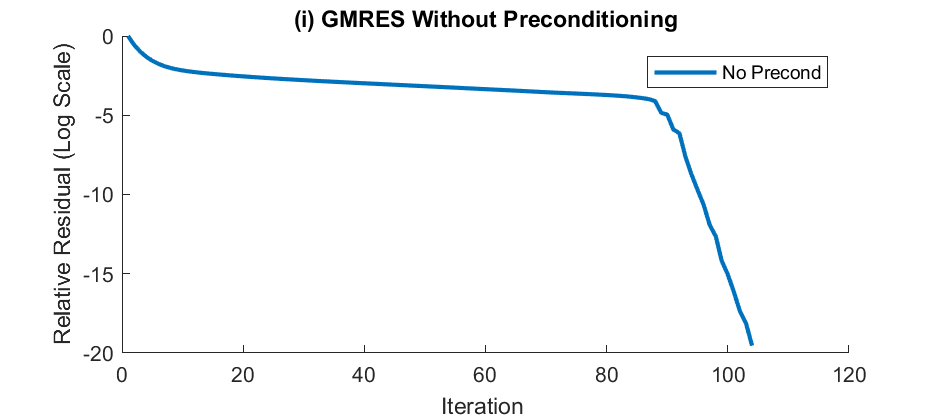
\includegraphics[width=0.49\textwidth]{../code/Mat1_1.png}}
   \subfloat{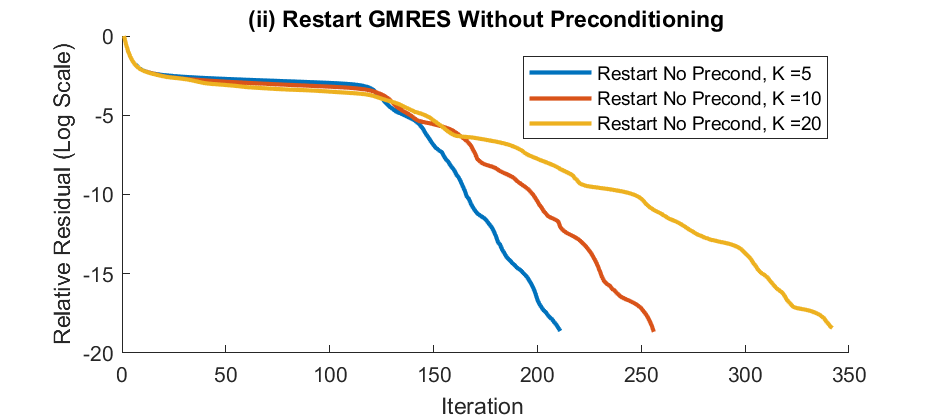
\includegraphics[width=0.49\textwidth]{../code/Mat1_2.png}}
      
   \subfloat{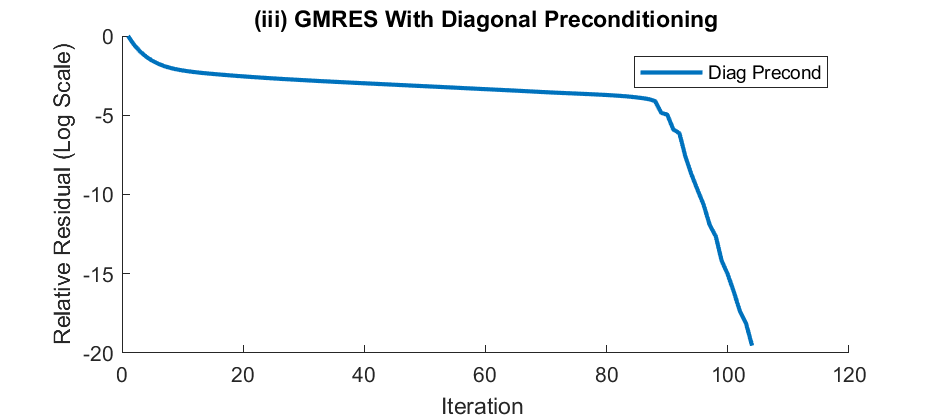
\includegraphics[width=0.49\textwidth]{../code/Mat1_3.png}}    
   \subfloat{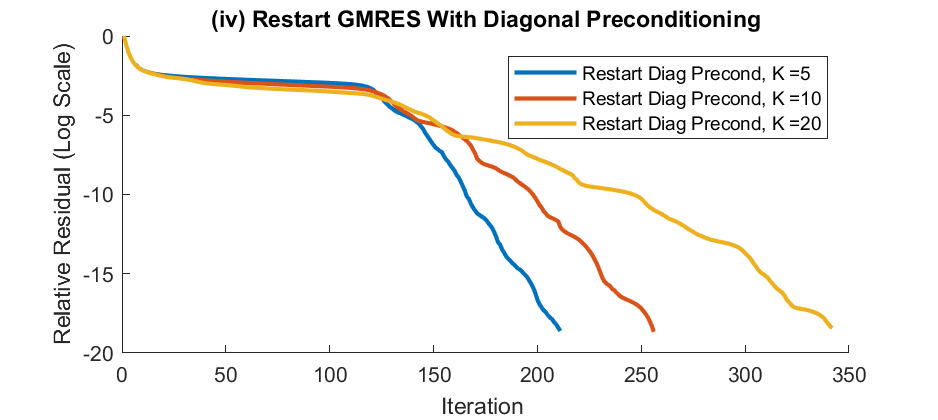
\includegraphics[width=0.49\textwidth]{../code/Mat1_4.png}}
   
   \subfloat{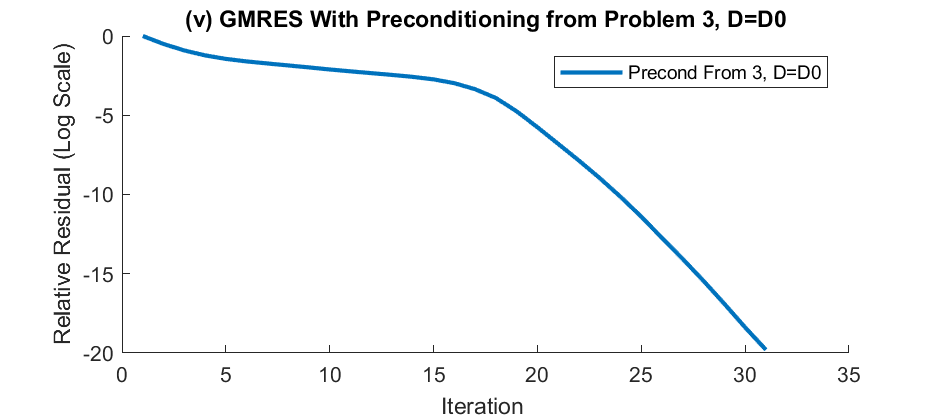
\includegraphics[width=0.49\textwidth]{../code/Mat1_5.png}}
   \subfloat{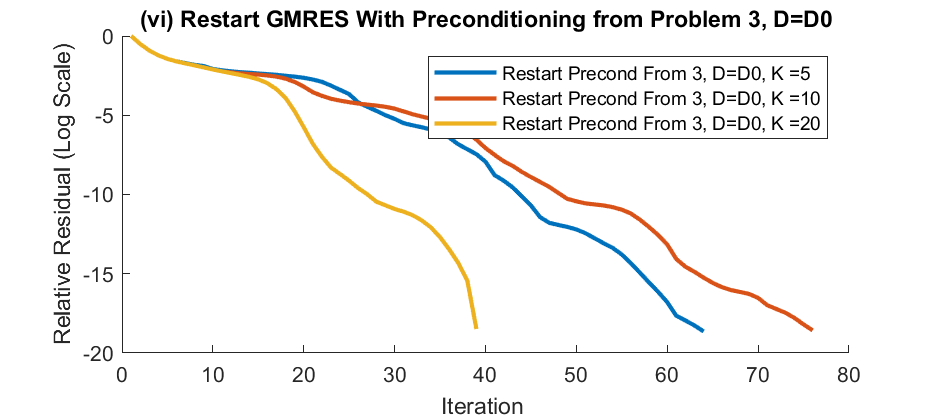
\includegraphics[width=0.49\textwidth]{../code/Mat1_6.png}}
   
   \subfloat{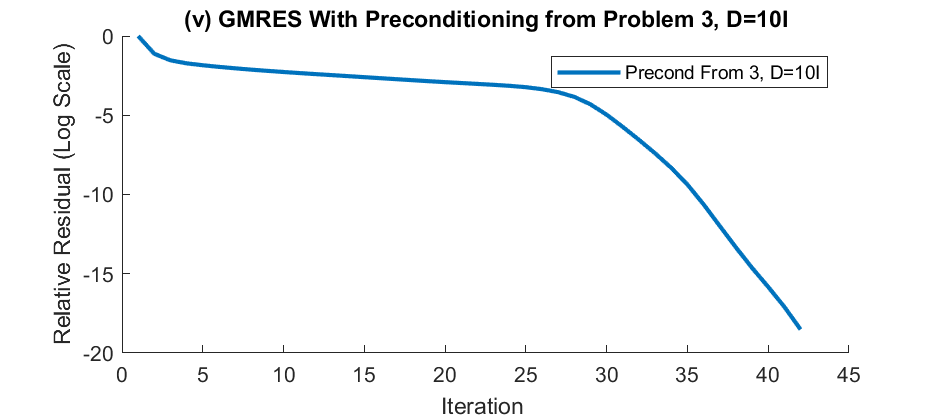
\includegraphics[width=0.49\textwidth]{../code/Mat1_7.png}}
   \subfloat{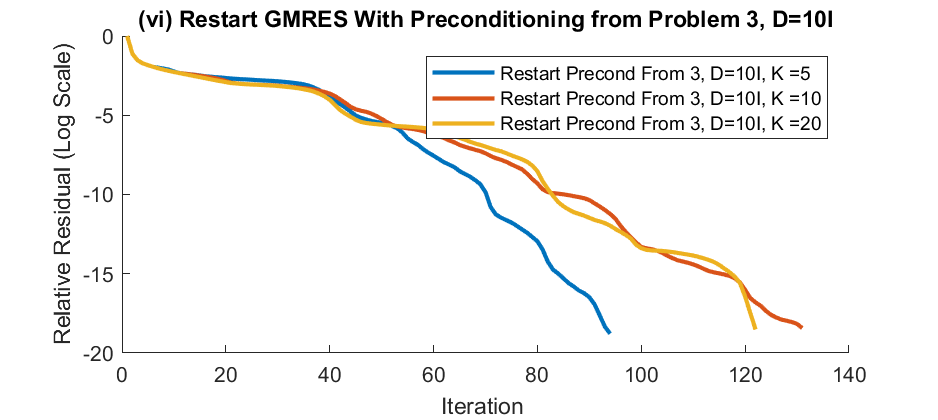
\includegraphics[width=0.49\textwidth]{../code/Mat1_8.png}}  

   \caption{Result for input matrix from \texttt{HW3_P4_1.mat}}
   \label{fig:mat1}
\end{figure}




\begin{figure}[tbh]
 \centering    
\begin{tabular}{ |p{6cm}|| p{1cm}|p{1.5cm}|p{1.5cm}|p{1.8cm}|p{1.7cm}|}
 \hline
Case & $k$ & Outer  & Inner &  \# GMRES  &\#  MatVec \\ \hhline{|=|=|=|=|=|=|}
 \hline
 (i) w/o Precondition                        &   &  1 & 192  & 193  & 194  \\
  \hline
 (ii) Restart w/o Precondition               & 5  & 67 & 4 & 335 & 402  \\                              
                                             & 10 & 40 & 7 & 398 & 438 \\
                                             & 20 & 25 & 2 & 483 & 508 \\                               
 \hline
(iii) Diagonal Precondition                  &   & 1 & 192 & 193 & 194 \\                              
 \hline
(iv) Restart Diagonal Precondition           & 5 & 67  & 4 & 335 & 402  \\                              
                                             & 10 & 40 & 7 & 398 & 438 \\
                                             & 20 & 25 & 2 & 483  & 508  \\
 \hline
(v) Precondition From 3, $D=D_{0}$           &   & 1 & 52 & 53 & 54 \\                              
 \hline
(v) Precondition From 3, $D=10I$             &   & 1 & 89 & 90 & 91  \\                              
 \hline
(vi) Restart Precondition From 3, $D=D_{0}$  & 5  & 24 & 2  & 118 & 142  \\                              
                                             & 10 & 15 & 1  & 142 & 157 \\
                                             & 20 & 10 & 15 & 196 & 206 \\
\hline
(vi) Restart Precondition From 3, $D=10I$    & 5  & 35 & 1 & 172 & 207  \\                              
                                             & 10 & 22 & 9 & 220 & 242  \\
                                             & 20 & 14 & 14& 275 & 289 \\
 \hline
\end{tabular} 
\caption{Results for input from \texttt{HW3_P4_2.mat}}
   \label{tab:mat2}
\end{figure} 

\begin{figure}[!tbh]
\centering        
   \subfloat{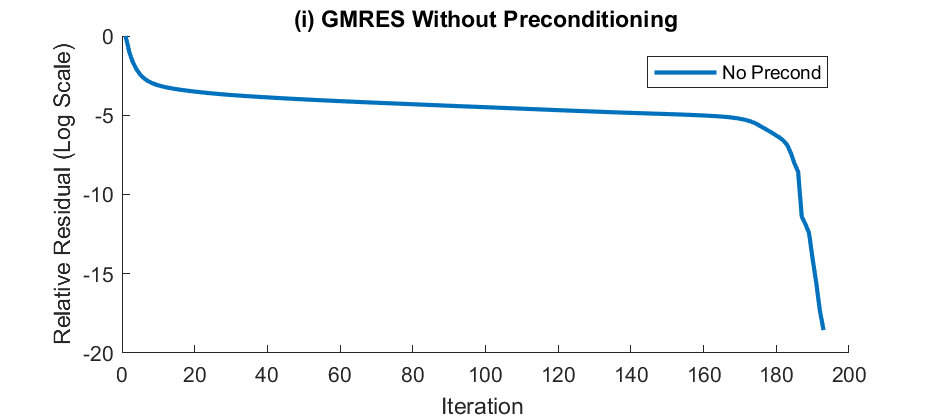
\includegraphics[width=0.52\textwidth]{../code/Mat2_1.png}}
   \subfloat{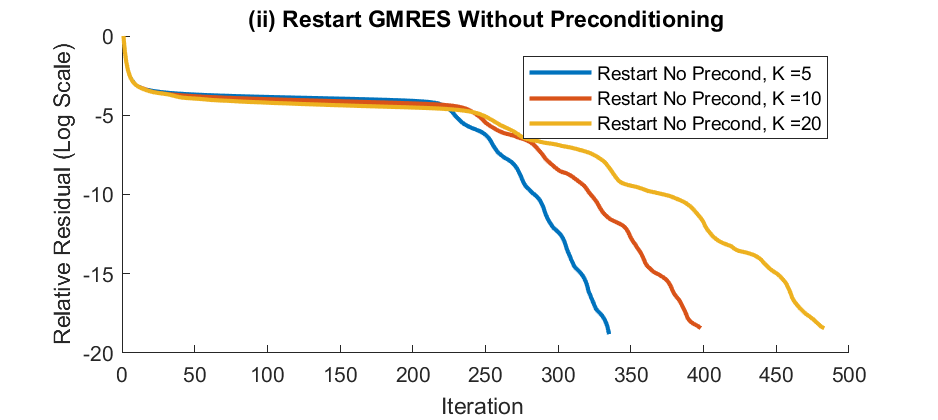
\includegraphics[width=0.52\textwidth]{../code/Mat2_2.png}}
      
   \subfloat{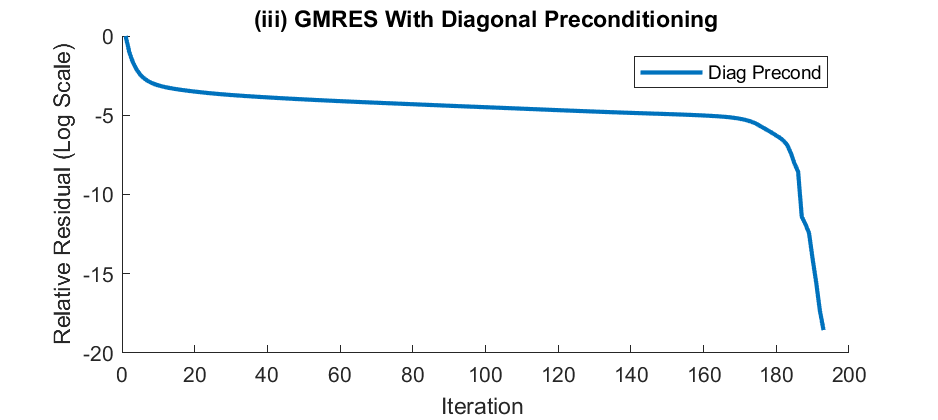
\includegraphics[width=0.52\textwidth]{../code/Mat2_3.png}}    
   \subfloat{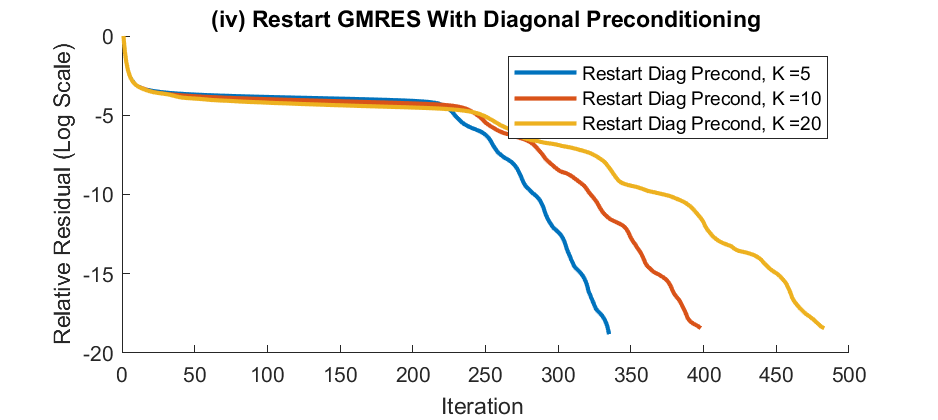
\includegraphics[width=0.52\textwidth]{../code/Mat2_4.png}}
   
   \subfloat{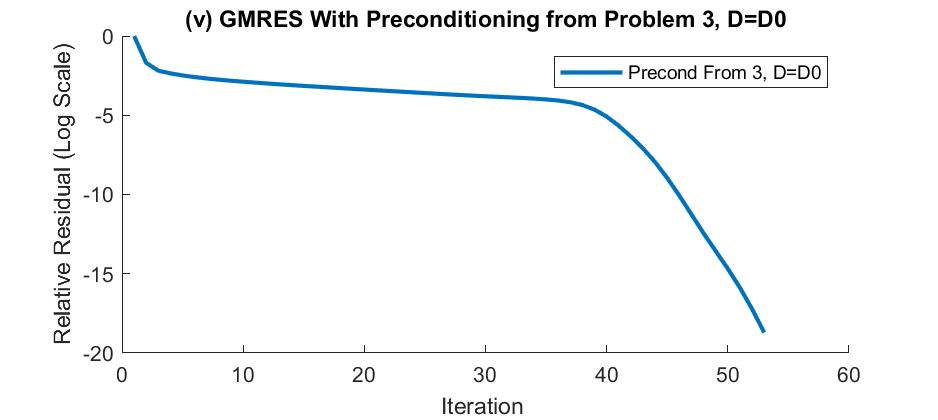
\includegraphics[width=0.52\textwidth]{../code/Mat2_5.png}}
   \subfloat{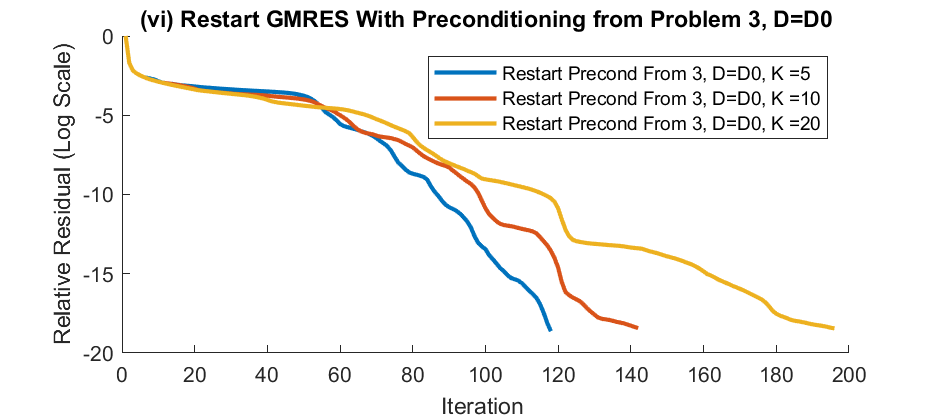
\includegraphics[width=0.52\textwidth]{../code/Mat2_6.png}}
   
   \subfloat{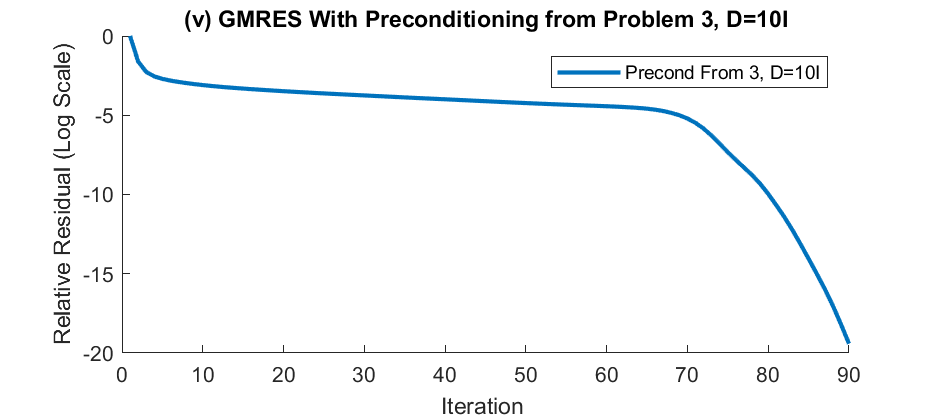
\includegraphics[width=0.52\textwidth]{../code/Mat2_7.png}}
   \subfloat{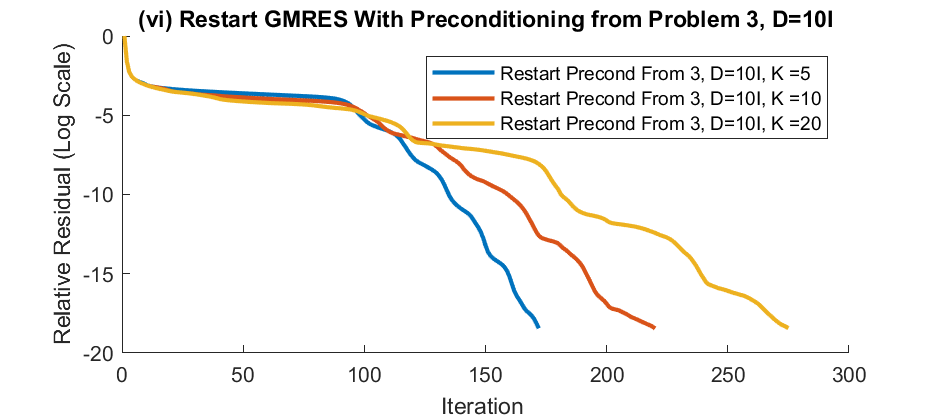
\includegraphics[width=0.52\textwidth]{../code/Mat2_8.png}}  

   \caption{Result for input matrix from \texttt{HW3_P4_2.mat}}
   \label{fig:mat2}
\end{figure}

\end{enumerate}